% Pregunta 4 - Ayudantía 8

\textbf{P4)} Una cuerda de 50.0 cm de longitud vibra sometida a una tensión de 1.00 N. La figura muestra cinco imágenes estroboscópicas sucesivas de la cuerda. La lámpara produce 5000 destellos por minuto y las observaciones revelan que el desplazamiento máximo se dio en los destellos 1 y 5, sin otros máximos intermedios.

\begin{center}
	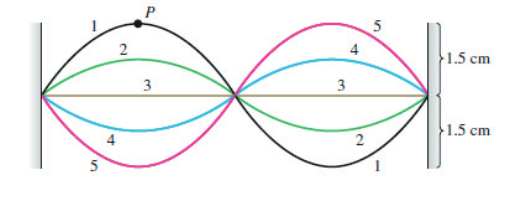
\includegraphics[width=0.65\textwidth]{../imagenes/imagen p4 a8.PNG}
\end{center}

a) Calcule la longitud de onda, el periodo y la frecuencia de las ondas que viajan por esta cuerda. 

b) ¿En qué modo normal (armónico) está vibrando la cuerda? 

c) Calcule la rapidez de las ondas viajeras en la cuerda. 

d) ¿Con qué rapidez se está moviendo el punto P cuando la cuerda está en i) la posición 1 y ii) la posición 3? 

e) Calcule la masa de la cuerda.

% Respuesta / espacio para soluciones

